\chapter{1T' $WSe_2$}

\section{Introduction}

The 1T and 1T' phases of group VI TMDCs have only recently gained significant attention compared to the more popular semiconducting 2H and number of reports in the literature has increased. They have been found to show promise in areas of electrocatalytic water splitting and energy storage thanks to lower charge transfer resistance\cite{Voiry2013}, a result of their metallic nature \cite{Wypych1992}. The 1T' phase is also predicted to be a large gap quantum spin Hall (QSH) insulator which can be useful in spintronic devices  application \cite{Chen2018}. In contrast to 1T' $WTe_2$ \cite{Fei2017} it can be used in ambient temperatures as well as ambient atmosphere unlike other known large gap QSH insulator materials like stanene \cite{Xu2013} or 2D In-Sb compounds \cite{Gruznev2018}. 

So far the synthesis of 1T and 1T' group VI sulfides and selenides ($MoS_2$, $WS_2$, $MoSe_2$, $WSe_2$)  phases has proven difficult due to the metastable nature of them. Most commonly a direct synthesis via e.g. a CVD route results in more thermodynamically stable 2H phase. The difference in energy per formula unit between 1H and 1T' $WSe_2$ phase is only 0.27 eV which suggests that under certain reaction conditions a metastable 1T' can be synthesised.

A colloidal synthesis has been attempted and flakes of varying thickness of $WSe_2$ has been achieved. 

\section{Results}

In order to ascertain the phase of the as grown $WSe_2$ a Raman spectrum has been taken. As seen in Figure \ref{fig:1T'RamanSpectrumPre} the spectrum looks very different to the Raman spectrum of 2H $WSe_2$ as seen in e.g. Figure \ref{fig:WSe2RamanSpectrum}. The $E^1_{2g}$ and $A_{1g}$ located around 250 $cm^{-1}$ and are convoluted in case of the monolayer. In Figure \ref{fig:1T'RamanSpectrumPre} the closest peaks to those are located at 248.6 and 260 $cm^{-1}$ and can be therefore ascribed to $E^1_{2g}$ and $A_{1g}$ modes respectively. Additionally the absence of the $B^1_{2g}$ peak suggest that the material is very thin. Furthermore there are 5 more unresolved peaks at 104.5, 149, 177, 218 and 236.3 $cm^{-1}$. Thus far there is no published information regarding the vibrational modes of 1T' $WSe_2$ and therefore the peaks cannot be assigned to the modes. Similarly new peaks have been reported for 1T' $MoS_2$ where new peaks were labelled as $J_1$, $J_2$ and $J_3$ \cite{Yu2018}.

\begin{figure}[!h]
	\begin{center}
		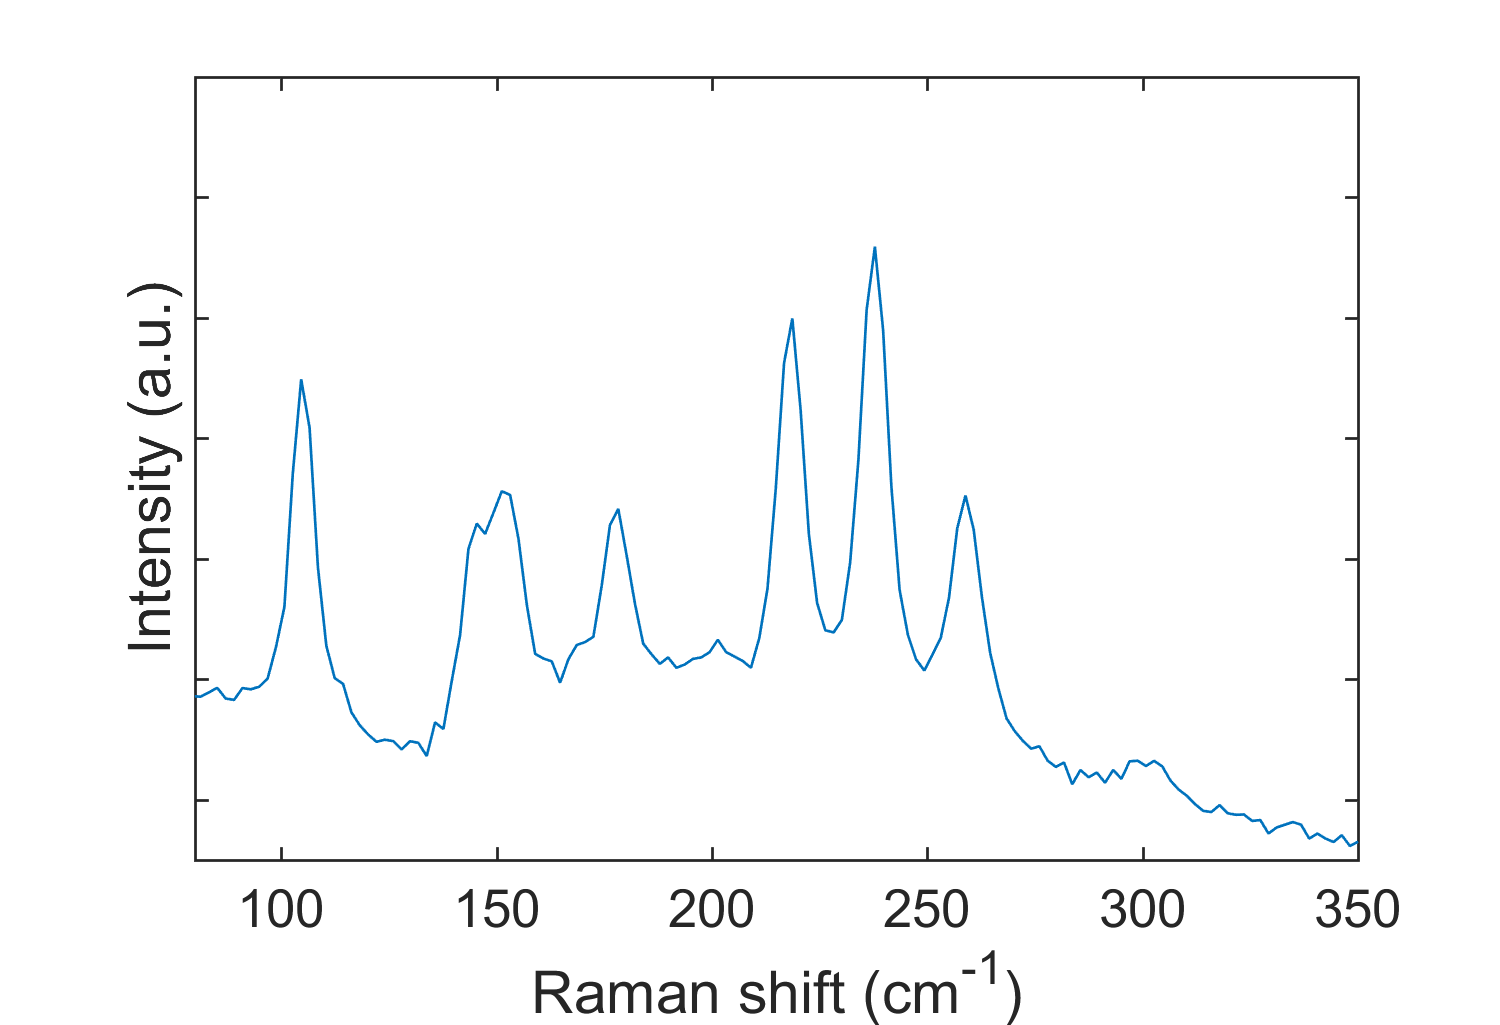
\includegraphics[scale=0.3]{1T'/RamanSpectrumPre.png}
		\caption{Raman spectrum of the as-grown $WSe_2$}
		\label{fig:1T'RamanSpectrumPre}
	\end{center}
\end{figure}

Similarly the XPS spectra were taken of the as-grown sample as seen in Figure \ref{fig:1T'XPSW4fPreSpectrum} and Figure \ref{fig:1T'XPSSe3dPreSpectrum}. The XPS spectrum of the W 4f electron shell shows a doublet of $W^{+4}$ 4f at 31.49 and 33.63 eV. This position varies notably from those reported for 2H $WSe_2$ and therefore are attributed to 1T' $WSe_2$.

\begin{figure}[!h]
	\begin{center}
		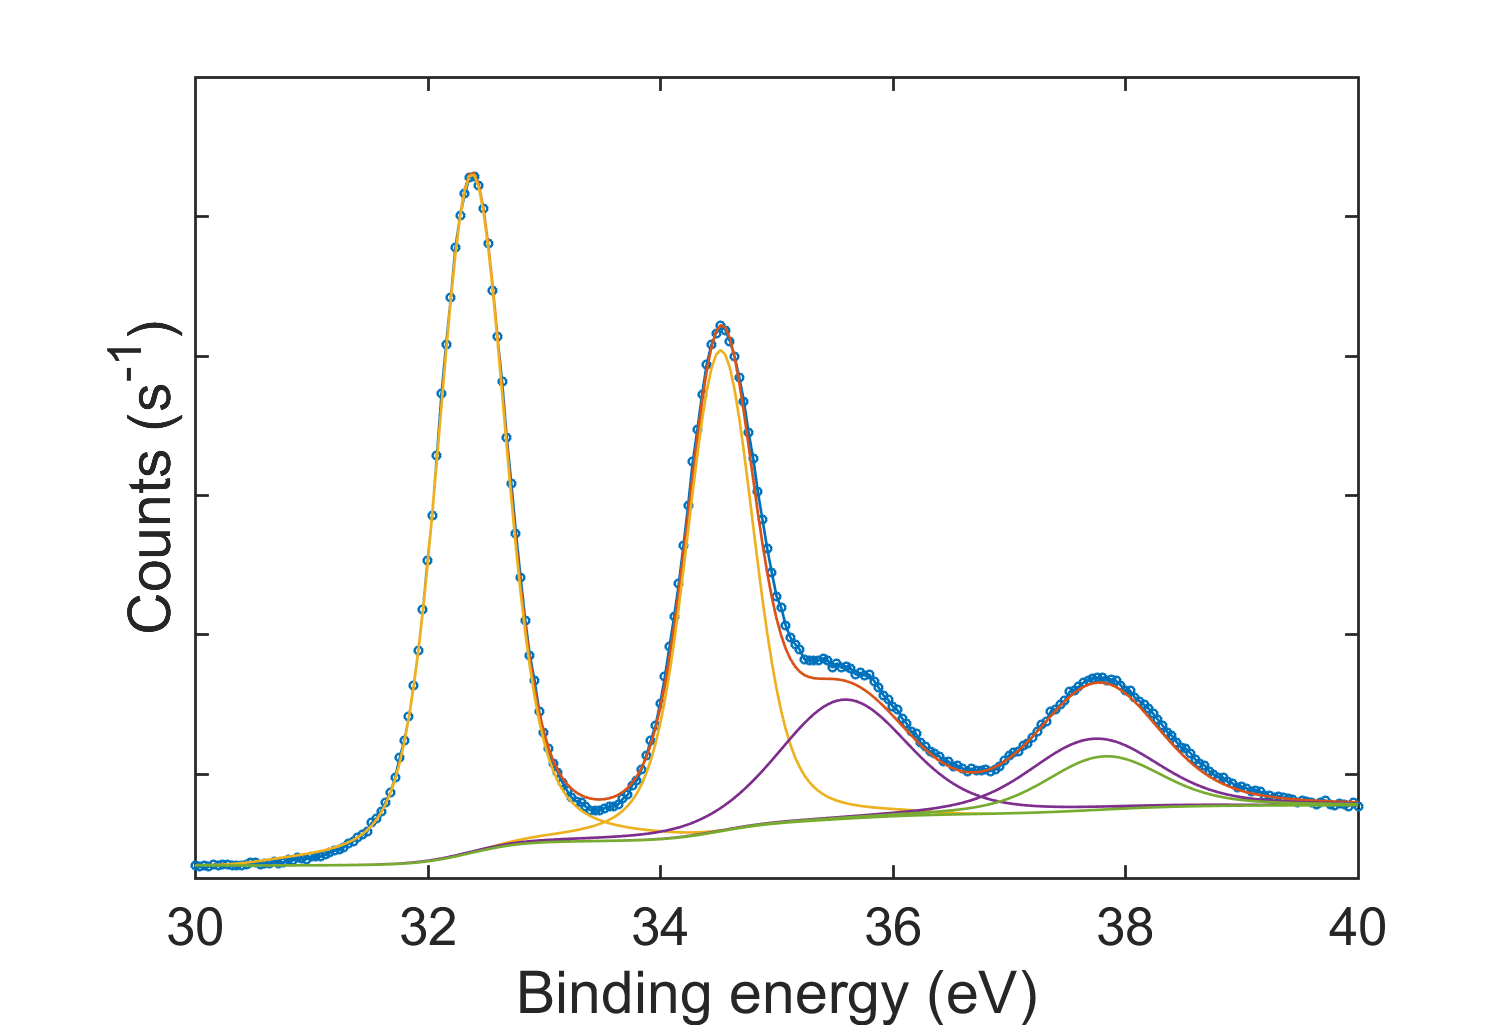
\includegraphics[scale=0.3]{1T'/XPSW4fPre.png}
		\caption{XPS Spectrum of W4f levels of the as-grown sample}
		\label{fig:1T'XPSW4fPreSpectrum}
	\end{center}
\end{figure}

\begin{figure}[!h]
	\begin{center}
		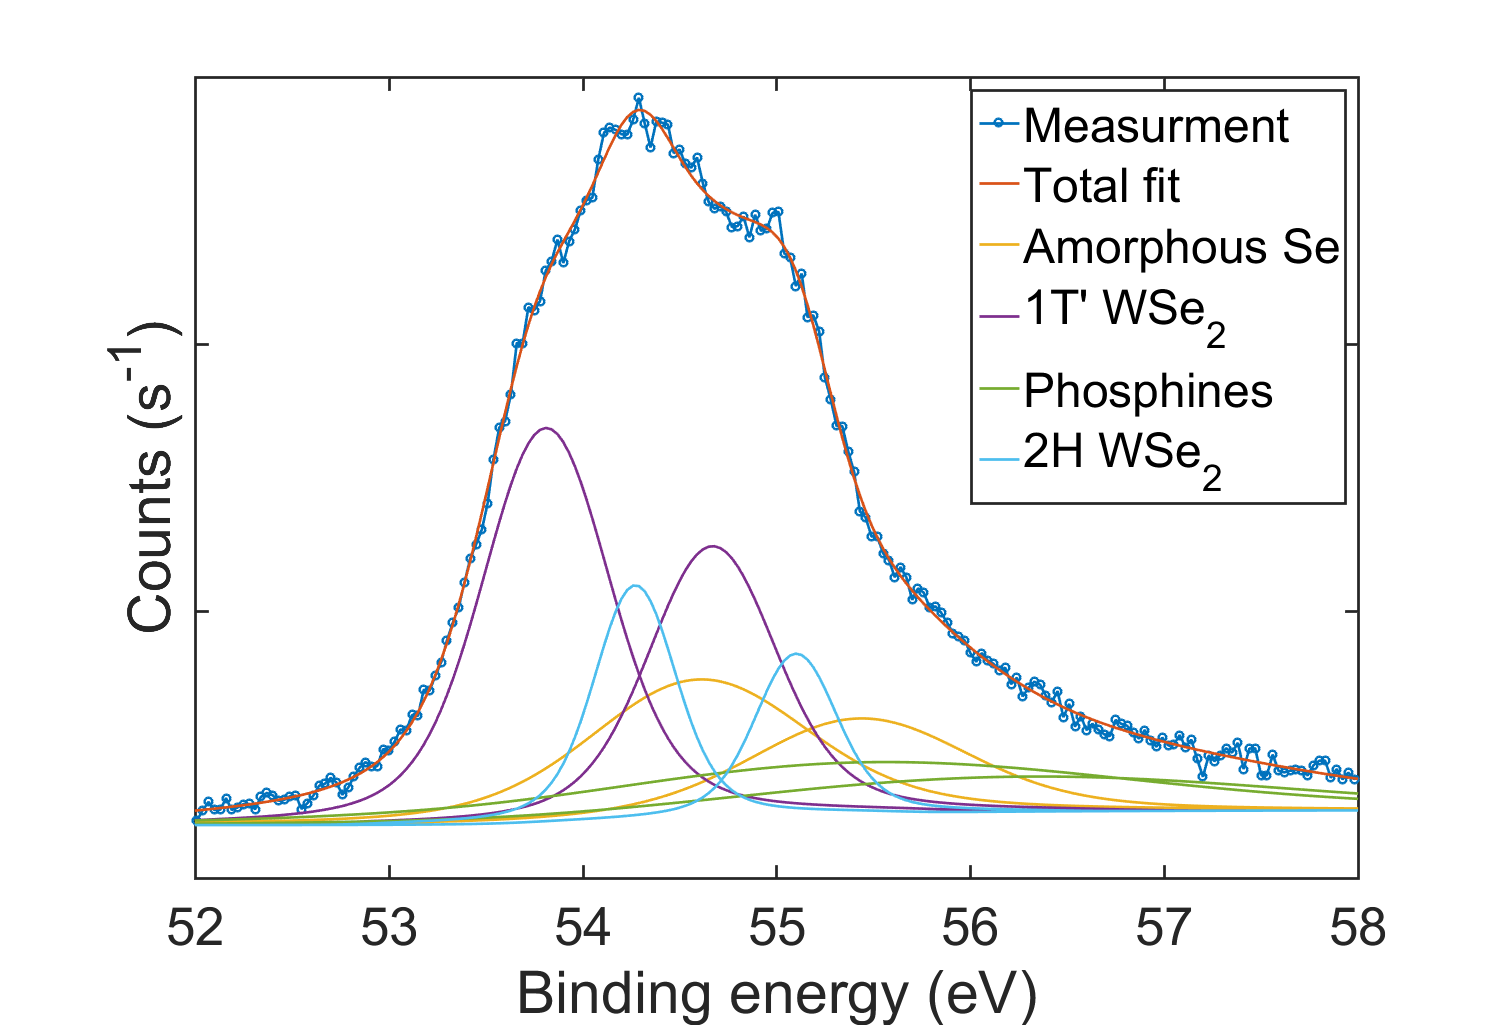
\includegraphics[scale=0.3]{1T'/XPSSe3dPre.png}
		\caption{XPS Spectrum of Se3d levels of the as-grown sample}
		\label{fig:1T'XPSSe3dPreSpectrum}
	\end{center}
\end{figure}

\begin{figure}[!h]
	\begin{center}
		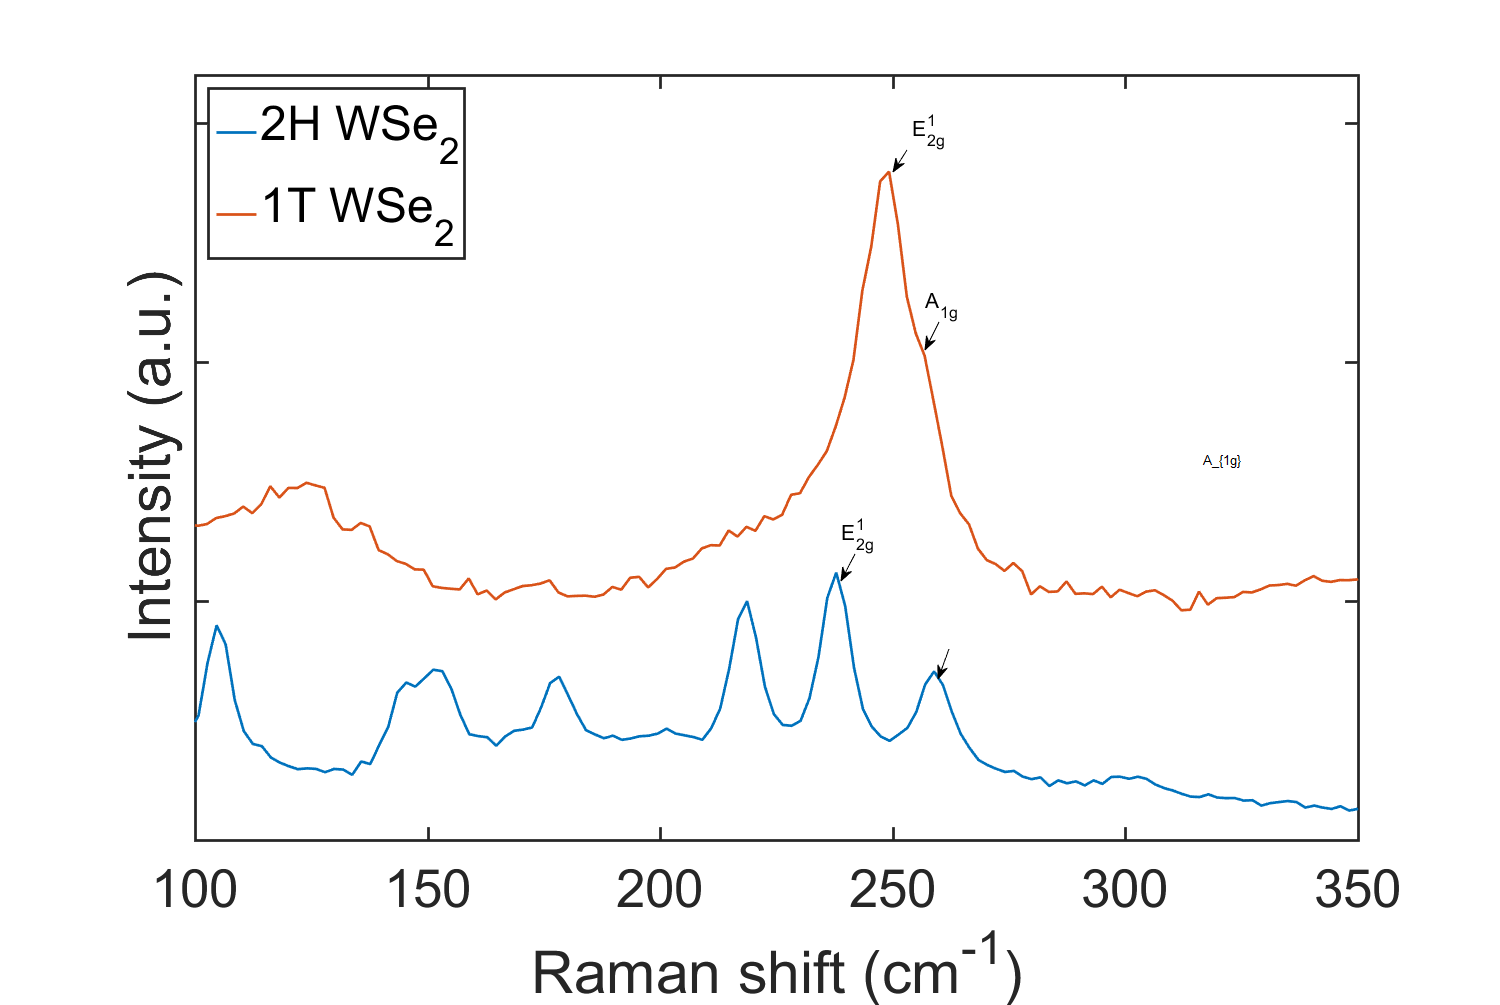
\includegraphics[scale=0.3]{1T'/RamanSpectraComparison.png}
		\caption{Raman spectra of 2H $WSe_2$ and 1T' $WSe_2$}
		\label{fig:1T'RamanSpectraComparison}
	\end{center}
\end{figure}